\section{Theorie}
\label{sec:Theorie}


\subsection{Allgemein}
Magnetfelder werden durch bewegte elektrische Ladungen hervorrufen. Der magnetische Fluss B wird in der Einheit Tesla 
angegeben und sowohl seine Richtung, als auch sein Betrag wird mithilfe der magnetischen Feldstärke $H$ beschrieben.
Zwischen der magnetischen Flussdichte B und der magnetischen Feldstärke H besteht der Zusammenhang

\begin{equation}
    \vec B = \mu \vec H,
    \label{eq:1}
\end{equation}
\noindent
wobei sich der Vorfaktor $\mu$ aus dem Produkt der Vakuum-Permeabilität $\mu_0$ und der stoffabhängigen relativen
Permeabilität $\mu_r$ zusammensetzt. Die relative Permeabilität ist lediglich dann relevant, wenn das Magnetfeld mit Materie 
wechselwirkt.


\subsection{Spulen}

Da bewegte Ladungen magnetische Felder hervorrufen, lässt sich auch um stromdurchflossene Leiter ein 
magnetisches Feld messen. Die magnetische Flussdichte B um eine beliebig geschlossene 
Leiterschleife lässt sich, mithilfe des Biot-Savart-Gesetzes
\begin{equation}
    d\vec B = \frac{\mu_0 I}{4 \pi} \frac{d\vec s \times \vec r}{r^3},
    \label{eq:2} 
\end{equation}
\noindent
im Abstand r berechnen. Mithilfe dieser Formel kann die magnetische Flussdichte auf einer Geraden, die durch den 
Mittelpunkt einer Leiterschleife verläuft und senkrecht zu dieser steht, ermittelt werden. Aus der Gleichung \ref{eq:2} ergibt sich 
\begin{equation}
    \vec B (x) = \frac{\mu_0 I}{2} \frac{R^2}{(R^2+x^2)^\frac{3}{2}} \hat{x},
\end{equation}
\noindent
wobei R der Radius des Ringes, x der Abstand zum Mittelpunkt auf der Symmetrieachse und $\hat{x}$ der Einheitsvektor ist,
der die Richtung des magnetischen Feldes angibt.
Liegt an Stelle eines Ringes eine Spule vor, so kann das Ergebnis mit der Windungszahl N multipliziert werden.

\subsection{Lange Spule}

Für den Fall, dass eine langegestreckte Spule mit $l \gg D$ vorliegt, so verlaufen die Feldlinien 
innerhalb dieser parallel zueinander, was bedeutet, dass die magnetische Flussdichte homogen 
ist und sich dessen Betrag mit der Formel
\begin{equation}
    B = \mu_r \mu_0 \frac{N}{l} I
    \label{eq:a}
\end{equation}
\noindent 
berechnen lässt, wobei deutlich wird, dass die magnetische Flussdichte sowohl zu der Stromstärke I, 
als auch zu der Windungszahl N proportional und zu der Spulenlänge l umgekehrt proportional ist.
Am Rand, ebenso wie außerhalb der Spule, ist das magnetische Feld inhomogen.

\subsection{Ringspule}

Falls eine Ringspule vorliegt, dessen Spulenradius R deutlich kleiner ist, als dessen Länge l, lässt sich
der Betrag der magnetischen Flussdichte B mit der Formel
\begin{equation}
    B = \mu_r \mu_0 \frac{N}{l} I
\end{equation}
\noindent
berechnen. Ebenso wie bei der langen Spule ist auch innerhalb der Ringspule das magnetische Feld
vollkommen homogen, allerdings ist außerhalb der Spule kein Magnetfeld vorhanden.


\subsection{Helmholtzspulen}

Um ein möglichst homogenes Magnetfeld zu erhalten, werden zwei identische Spulen mit dem Radius R und der Windungszahl N 
so aufgestellt, dass die Verbindungslinie der Spulenmittelpunkte senkrecht zu den Spulen selbst steht. Wird der Abstand 
der Spulen so eingestellt, dass dieser dem Radius R entspricht, so ergibt sich auf der Verbindungslinie der 
Spulenmittelpunkte ein homogenes Magnetfeld, für das sich die magnetische Flussdichte im Mittelpunkt der Spulen durch
die Überlagerung der einzelnen Felder ergibt. 
Weicht der Abstand der Spulen zueinander von dem Wert R ab, so ergibt sich der Wert für den magnetischen Fluss B im 
Mittelpunkt von zwei Spulen mit je einer Windung durch die Gleichung
\begin{equation}
    B(0) = B_1(x) + B_1(-x) = \frac{\mu_0 I R^2}{(R^2 + x^2)^{\frac{3}{2}}},
    \label{eq:b}
\end{equation}
\noindent
wobei der Nullpunkt so gewählt ist, dass der Mittelpunkt der Helmholtzspulen in ihm liegt und der Wert x 
der Hälfte des Abstandes der Spulen zueinander entspricht.

\subsection{Hysteresekurve}

\noindent
Bedingt dadurch, dass bei Ferromagneten die relative Permeabilität $\mu_r \gg 1$ ist, verliert Gleichung \ref{eq:1}
ihre Gültigkeit. Um den Zusammenhang zwischen magnetischer Erregung und magnetischem Fluss dennoch darstellen zu können, wird
eine sogenannte Hysteresekurve erstellt. Diese gibt auf der x-Achse den Wert der magnetischen Feldstärke und auf der y-Achse
den Wert der magnetischen Flussdichte an. \\

Wird ein ferromagnetisches Material, welches noch nicht magnetisiert ist, zum ersten Mal durch ein äußeres
Magnetfeld beeinflusst, vergrößern sich die Weißschen Bezirke (siehe \ref{sec:v}), bis alle magnetischen Momente in dieselbe Richtung zeigen.
In diesem Punkt ist der magnetische Fluss am größten. Es wird im Allgemeinen von der Sättigungsmagnetisierung $B_S$ gesprochen.
Weiterhin wird der Kurvenverlauf vom Ursprung bis zur Sättigungsmagnetisierung Neukurve genannt.
\begin{figure}[H]
    \centering
    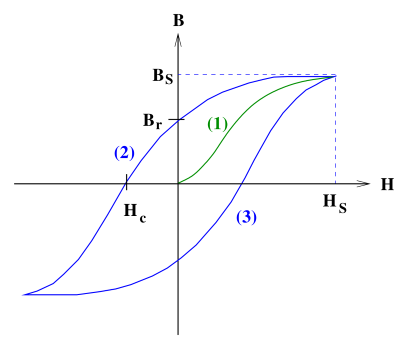
\includegraphics{content/Bild1.png}
    \caption{Darstellung einer allgemeinen Hysteresekurve (blau) samt Neukurve (grün) \cite {sample}}
    \label{Hysteresekurve}
\end{figure}
\noindent
Wenn das äußere Magnetfeld nun stufenweise abgeschaltet wird, verbleibt der Ferromagnet weiterhin in einem
magnetisierten Zustand. In diesem Fall wird der Wert für den magnetischen Fluss wird als Remanenz $B_r$ bezeichnet.
Durch das Anlegen eines Magnetfeldes, welches antiparallel zu dem 
zuerst angelegten Feld verläuft, kann das Material wieder in einen unmagnetisierten Zustand gebracht werden. Der hier gemessenen Wert 
für die magnetische Feldstärke H wird allgemein Koerzitivkraft $H_c$ genannt. Das äußere Magnetfeld kann nun gleichmäßig herauf- und anschließend wieder herabgefahren werden.
Abgesehen von dem Vorzeichen ergeben sich dieselben Werte für die Sättigungsmagnetisierung beziehungsweise die Remanenz. Um die Hysteresekurve
zu vervollständigen kann das äußere Feld ein weiteres Mal umgepolt und schrittweise erhöht werden, sodass sich abermals die Sättigungsmagnetisierung
ergibt. 
\\
Es ist zu beachten, dass der Zustand des Ferromagneten nicht nur von dem außen angelegten Feld abhängig ist, sondern auch
von der Vorgeschichte des Materials. Zusätzlich fällt auf, dass die Hysteresekurve symmetrisch zum Ursprung verläuft.


\subsection{Vorbereitungsaufgaben}
\label{sec:v}
Als Diamagnet wird ein Material bezeichnet, welches ohne den Einfluss eines 
äußeren magnetischen Feldes in einem völlig unmagnetisierten Zustand verbleibt.
Durch den Einfluss eines äußeren Magnetfeldes richten sich die magnetischen 
Momente innerhalb des Materials so aus, dass sie antiparallel zum äußeren 
Feld zeigen. Somit entsteht ein Magnetfeld, welches einen betragsmäßig kleineren 
Wert besitzt, als das Feld ohne Diamagnet.

Als Paramagnet wird ein Material bezeichnet, dass genauso wie der Diagmagnet 
ohne den Einfluss von einem äußeren Magnetfeld in einem vollkommen unmagnetiserten
Zustand verbleibt. Durch den Einfluss eines äußeren magnetischen Feldes richten 
sich die magnetischen Momente innerhalb des Materials so aus, dass sie parrallel 
zum äußeren Feld zeigen. Es ensteht also ein Magnetfeld, welches einen betragsmäßig 
größeren Wert besitzt, als das Feld ohne Paramagnet.

Im Gegensatz zu Dia- und Paramagneten besitzen Ferromagneten bereits ohne ein von außen angelegtes Magnetfeld
ein permanentes magnetisches Moment. Innerhalb von sogenannten Weißschen Bezirken verlaufen die magnetischen Momente
parallel, allerdings sind diese Bereiche statistisch über den gesamten Körper verteilt und heben sich gegenseitig auf,
sodass der Körper als ganzes kein magnetisches Feld besitzt. Wird nun ein äußeres Magnetfeld eingeschaltet, so ändert 
sich die Ausrichtung der einzelnen magnetischen Momente und die Weißschen Bezirke vergrößern sich. Das äußere Magnetfeld 
lässt sich so weit erhöhen, bis alle magnetischen Momente die gleiche Ausrichtung aufweisen. 
